\begin{frame}{Shellcode}{Definition}
    \begin{itemize}
        \item Shellcode ist eine Folge von Anweisungen. \\
        Diese kann über einen Exploit in einen Prozess injiziert werden.
        \item In der Computersicherheit meint Shellcode ursprünglich Code,
        der bei der Ausführung eine Shell öffnet
        \item Üblicherweise in Assembly
    \end{itemize}
\end{frame}


\begin{frame}{Shellcode}{Beispiel}
    \begin{figure}[h]
        \centering
        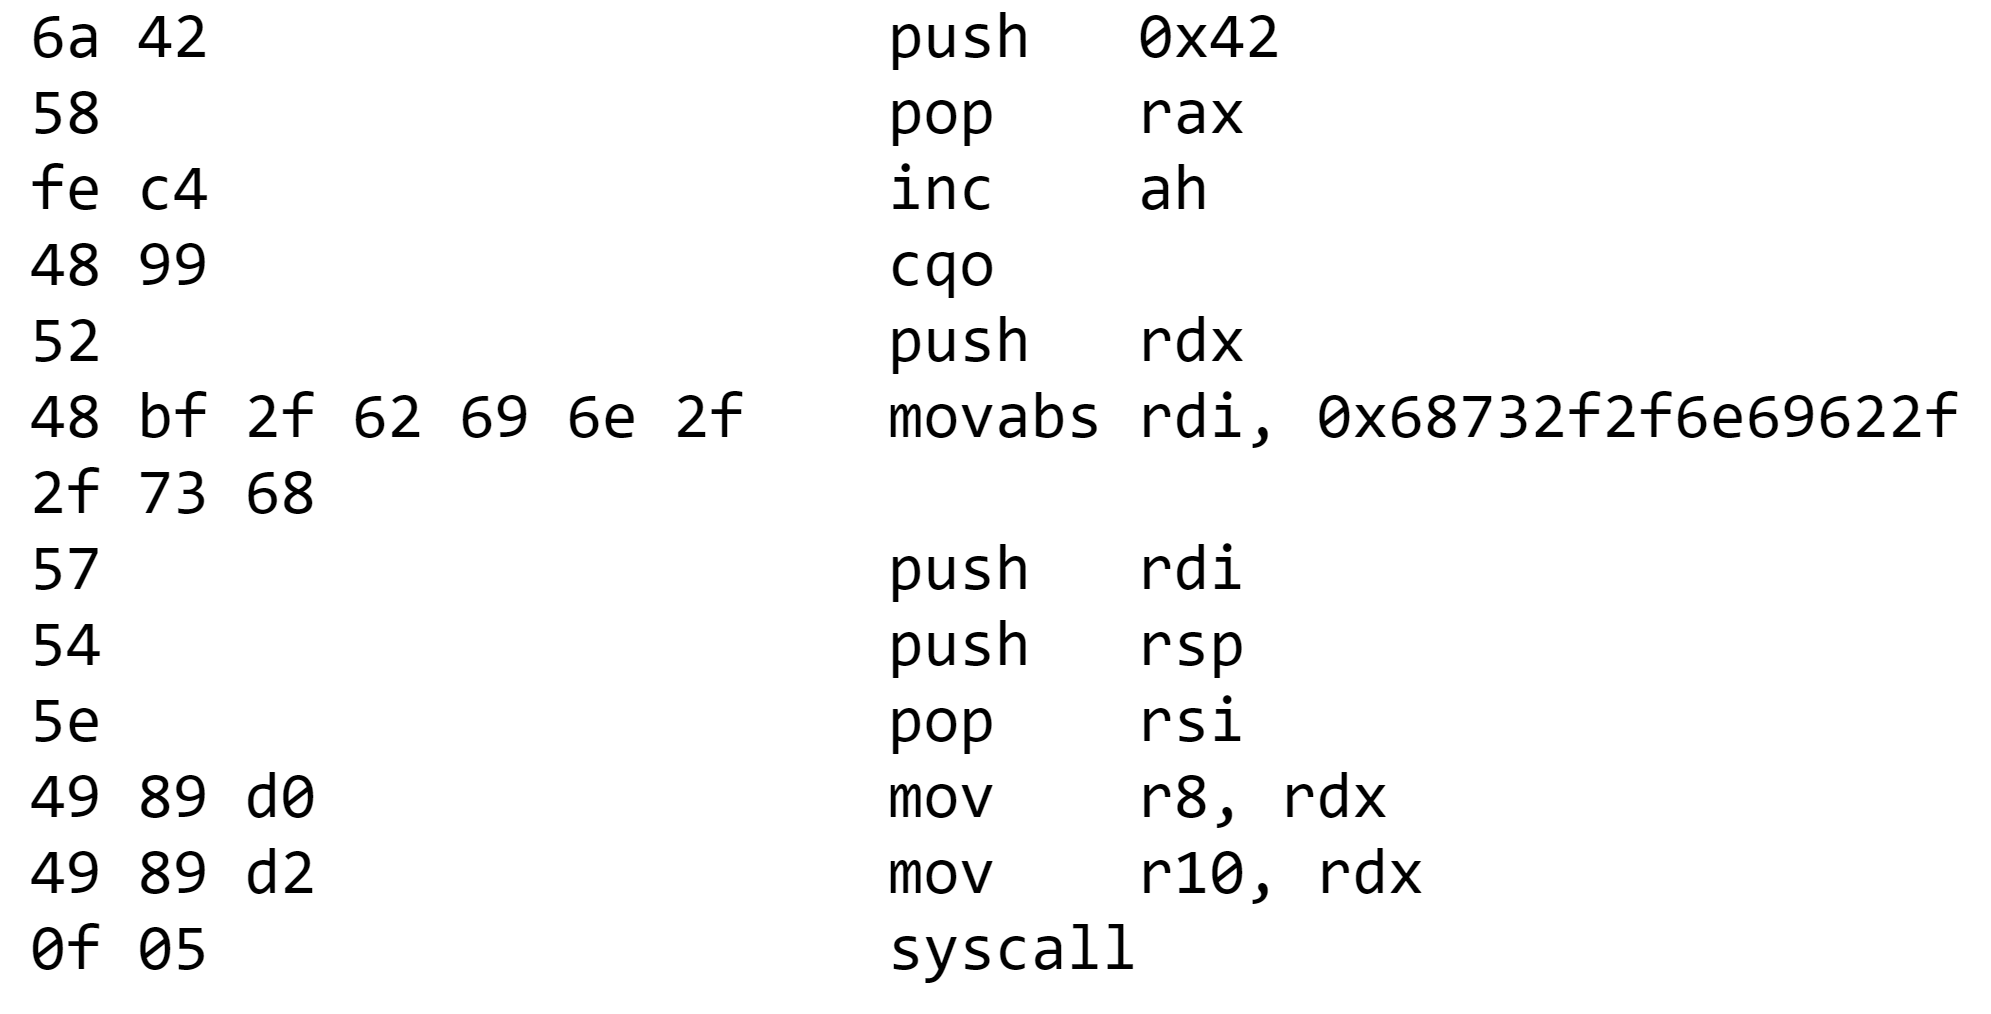
\includegraphics[width=0.9\textwidth,height=0.75\textheight,keepaspectratio]{images/shellstorm.png}
    \end{figure}
\end{frame}

\begin{frame}{Shellcode}{Register zum Zeitpunkt des Syscalls}
    Die verwendeten Register:
    
    \begin{tabular}{rl}
        {\textbf{RAX}:}& {322 (Nummer des Syscalls)}\\
        {\textbf{RDI}:}& {0x68732f2f6e69622f (Pfad der auszuführenden Datei: ''/bin//sh'')}\\
        {\textbf{RSI}:}& {Pointer auf RDI (Zeiger auf den Pfad)}
    \end{tabular}
    \vspace{1em}
    
    Die optionalen bzw. nicht verwendeten Register:
    
    \begin{tabular}{rl}
        {\textbf{RDX}:}& {0 (Optional)}\\
        {\textbf{R10}:}& {0 (Optional)}\\
        {\textbf{R8}:}& {0 (Optional)}\\
        {\textbf{R9}:}& {? (Nicht verwendet)}
    \end{tabular}

\end{frame}